\let\negmedspace\undefined
\let\negthickspace\undefined
\documentclass[journal]{IEEEtran}
\usepackage[a5paper, margin=10mm, onecolumn]{geometry}
%\usepackage{lmodern} % Ensure lmodern is loaded for pdflatex
\usepackage{tfrupee} % Include tfrupee package

\setlength{\headheight}{1cm} % Set the height of the header box
\setlength{\headsep}{0mm}     % Set the distance between the header box and the top of the text

\usepackage{gvv-book}
\usepackage{gvv}
\usepackage{cite}
\usepackage{amsmath,amssymb,amsfonts,amsthm}
\usepackage{algorithmic}
\usepackage{graphicx}
\usepackage{textcomp}
\usepackage{xcolor}
\usepackage{txfonts}
\usepackage{listings}
\usepackage{enumitem}
\usepackage{mathtools}
\usepackage{gensymb}
\usepackage{comment}
\usepackage[breaklinks=true]{hyperref}
\usepackage{tkz-euclide} 
% \usepackage{gvv}                                        
\def\inputGnumericTable{}                                 
\usepackage[latin1]{inputenc}                                
\usepackage{color}                                            
\usepackage{array}                                            
\usepackage{longtable}                                       
\usepackage{calc}                                             
\usepackage{multirow}                                         
\usepackage{hhline}                                           
\usepackage{ifthen}                                           
\usepackage{lscape}
\begin{document}

\bibliographystyle{IEEEtran}
\vspace{3cm}

\title{12.6.6.14}
\author{EE24BTECH11029 - J SHRETHAN REDDY}
\maketitle
% \newpage
% \bigskip
{\let\newpage\relax\maketitle}

\renewcommand{\thefigure}{\theenumi}
\renewcommand{\thetable}{\theenumi}
\setlength{\intextsep}{10pt} % Space between text and floats


\numberwithin{equation}{enumi}
\numberwithin{figure}{enumi}
\renewcommand{\thetable}{\theenumi}
\textbf{Question}:\\
Find the absolute maximum and minimum values of the function f given by\\
$f\brak{x}= \cos^2 x+\sin x,x\in \sbrak{0,\pi}$\\
\textbf{Answer}\\
\textbf{Theoritical Solution}\\
\begin{align}
    f\brak{x}&= \cos^2 x+\sin x\\
    f^\prime\brak{x}&=-\sin{2x}+\cos{x}\\
    f^\prime\brak{x}&=\cos{x}\brak{1-2\sin{x}}
\end{align}
solve $f^\prime\brak{x}=0$\\
\begin{align}
    \cos{x}=0 \quad or \quad 1-2\sin{x}=0
\end{align}
Case $1\colon\cos{x}=0$
\begin{align}
    x=\frac{\pi}{2}
\end{align}
Case $2\colon1-2\sin{x}=0$
\begin{align}
    x=\frac{\pi}{6} \quad or x=\frac{5\pi}{6}
\end{align}
critical points are $x=\frac{\pi}{6},\frac{\pi}{2},\frac{5\pi}{6}$\\
endpoints are $x=0,\pi$
Evaluation of $f\brak{x}$ at critical points and endpoints.\\
At $x=0$
\begin{align}
    f\brak{0}&=\cos^2{0}+\sin{0}=1
\end{align}
At $x=\pi$
\begin{align}
    f\brak{\pi}&=\cos^2{\pi}+\sin{\pi}=1
\end{align}
At $x=\frac{\pi}{2}$\\
\begin{align}
    f\brak{\frac{\pi}{2}}&=\cos^2{\frac{\pi}{2}}+\sin{\frac{\pi}{2}}\\
    f\brak{\frac{\pi}{2}}&=1
\end{align}

At $x=\frac{\pi}{6}$\\
\begin{align}
    f\brak{\frac{\pi}{6}}&=\cos^2{\frac{\pi}{6}}+\sin{\frac{\pi}{6}}\\
    &=\brak{\frac{\sqrt{3}}{2}}^2+\frac{1}{2}\\
        f\brak{\frac{\pi}{6}}&=\frac{5}{4}
\end{align}
At $x=\frac{5\pi}{6}$
\begin{align}
    f\brak{\frac{5\pi}{6}}&=\cos^2{\frac{5\pi}{6}}+\sin{\frac{5\pi}{6}}\\
    &=\brak{-\frac{\sqrt{3}}{2}}^2+\frac{1}{2}\\
    f\brak{\frac{5\pi}{6}}&=\frac{5}{4}
\end{align}
absolute maxima is $\frac{5}{4}$ at $x=\frac{\pi}{6},\frac{5\pi}{6}$\\
absolute minima is $1$ at $x=0,\frac{\pi}{2},\pi$\\
\textbf{Numerical method}  \\

Finding maximum and minimum value of function can be done using \textbf{Gradient Ascent and Descent method} \\
maximum value \\
\begin{align}
    x_{n+1}&=x_n+\alpha f^\prime\brak{x}\\
    x_{n+1}&=x_{n}+\alpha\brak{\cos{x}\brak{1-2\sin{x}}}
\end{align}
minimum value\\
\begin{align}
     x_{n+1}&=x_n-\alpha f^\prime\brak{x}\\
    x_{n+1}&=x_{n}-\alpha\brak{\cos{x}\brak{1-2\sin{x}}}
\end{align}
Where $\alpha$ is learning rate. Taking \\
\begin{align}
    h&=0.001\\
    \alpha&=0.001
\end{align}
we have
\begin{align}
    x_{max}=0.5230988543174608, y_{max}=1.2499998125049454\\
    x_{min}=1.5702963169279682, y_{min}=1.0000001250049153
\end{align}

 \begin{figure}[h!]
    \centering
    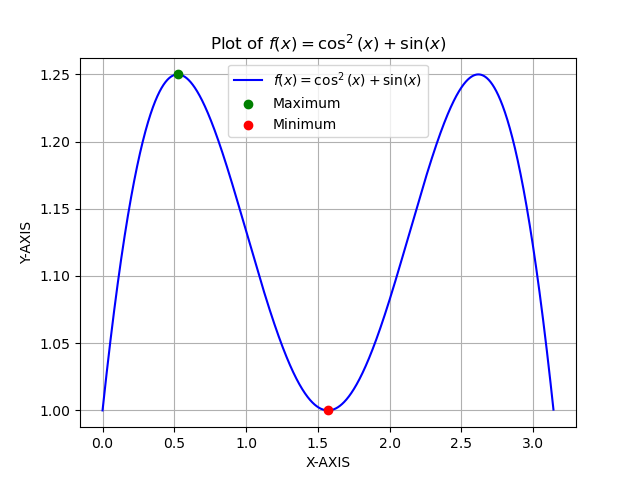
\includegraphics[width=1\columnwidth]{figure/fig.png} 
    \caption{plot}
    \label{stemplot}
 \end{figure}

\end{document}
